\chapter{Výstup skriptů pro vytvoření databáze}
\label{ch:appendix-database-scripts-output}

% Hackerman, hihi
\vspace{-4em}

\begin{figure}[ht]
    \centering
    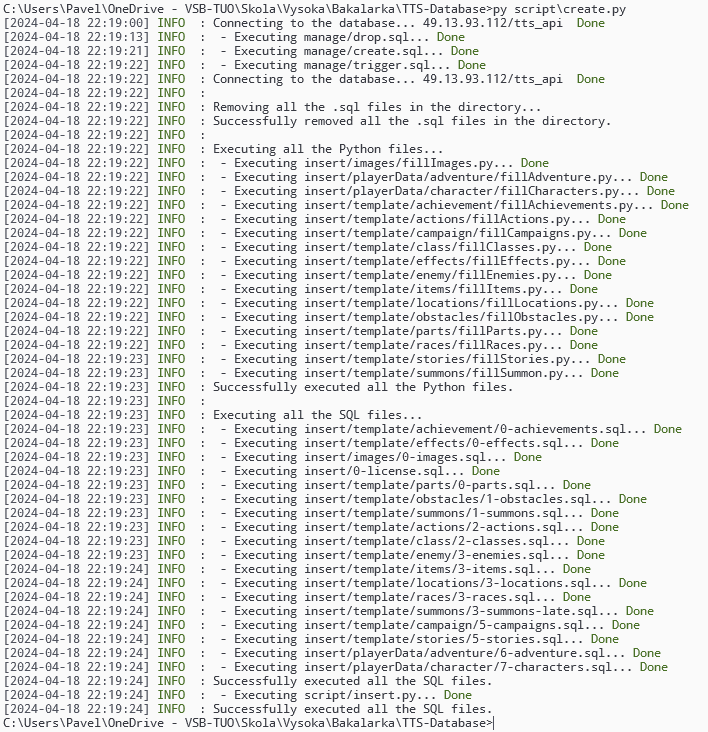
\includegraphics[width=0.95\textwidth]{figures/dbScriptsOutput}
    \caption{Výstup skriptů pro vytvoření databáze.}
    \label{fig:databaseScriptsOutput}
\end{figure}

\chapter{Ukázka rozhraní}
\label{ch:appendix-interface-screenshots}

% Hackerman again, hihi
\vspace{-4em}

\begin{figure}[ht]
    \centering
    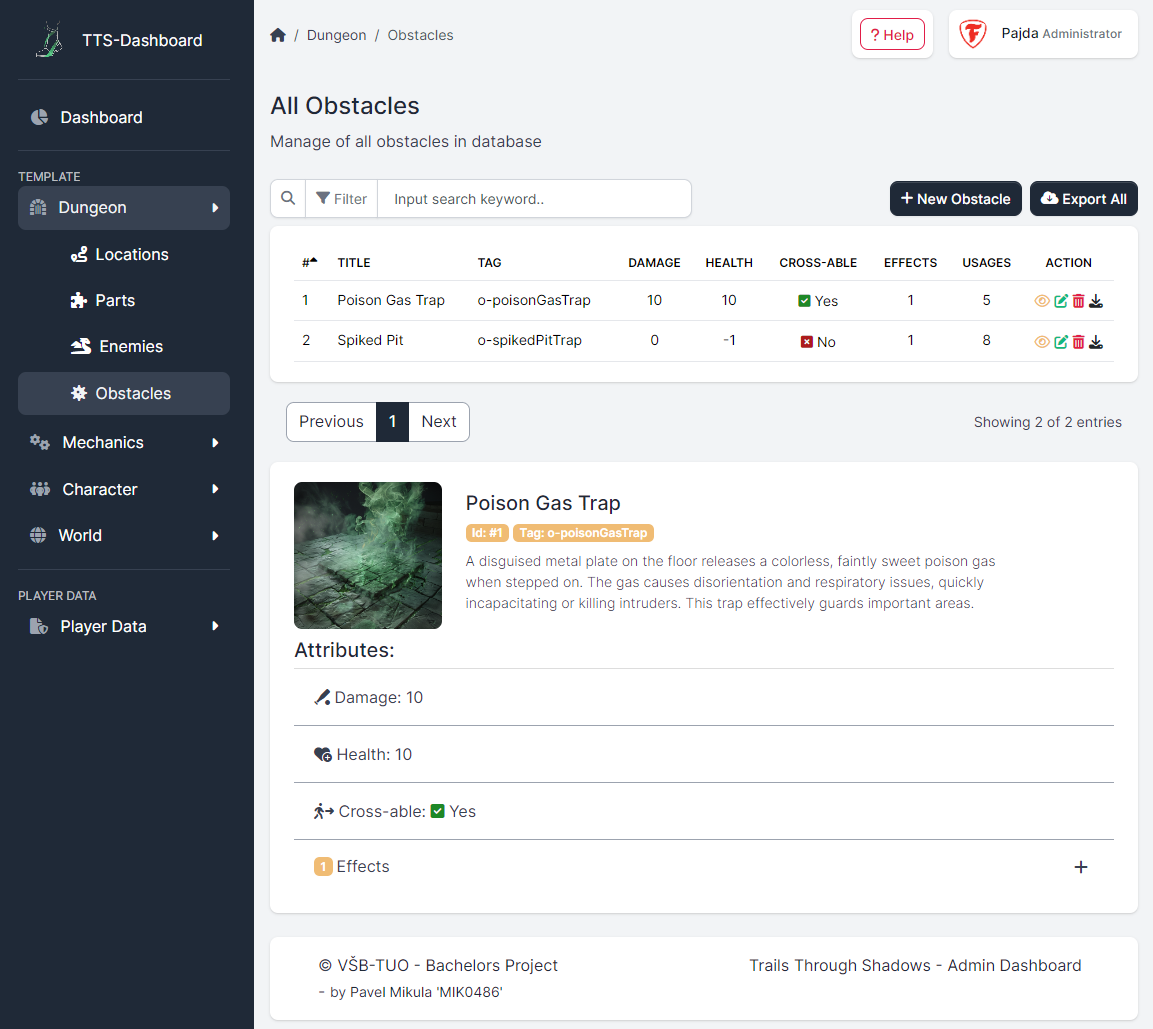
\includegraphics[width=0.95\textwidth]{figures/dashboardTableHorizontal}
    \caption{Ukázka výslédného rozhraní horizontální.}
    \label{fig:interfaceScreenshotsTableHorizontal}
\end{figure}

\begin{sidewaysfigure}[ht]
    \centering
    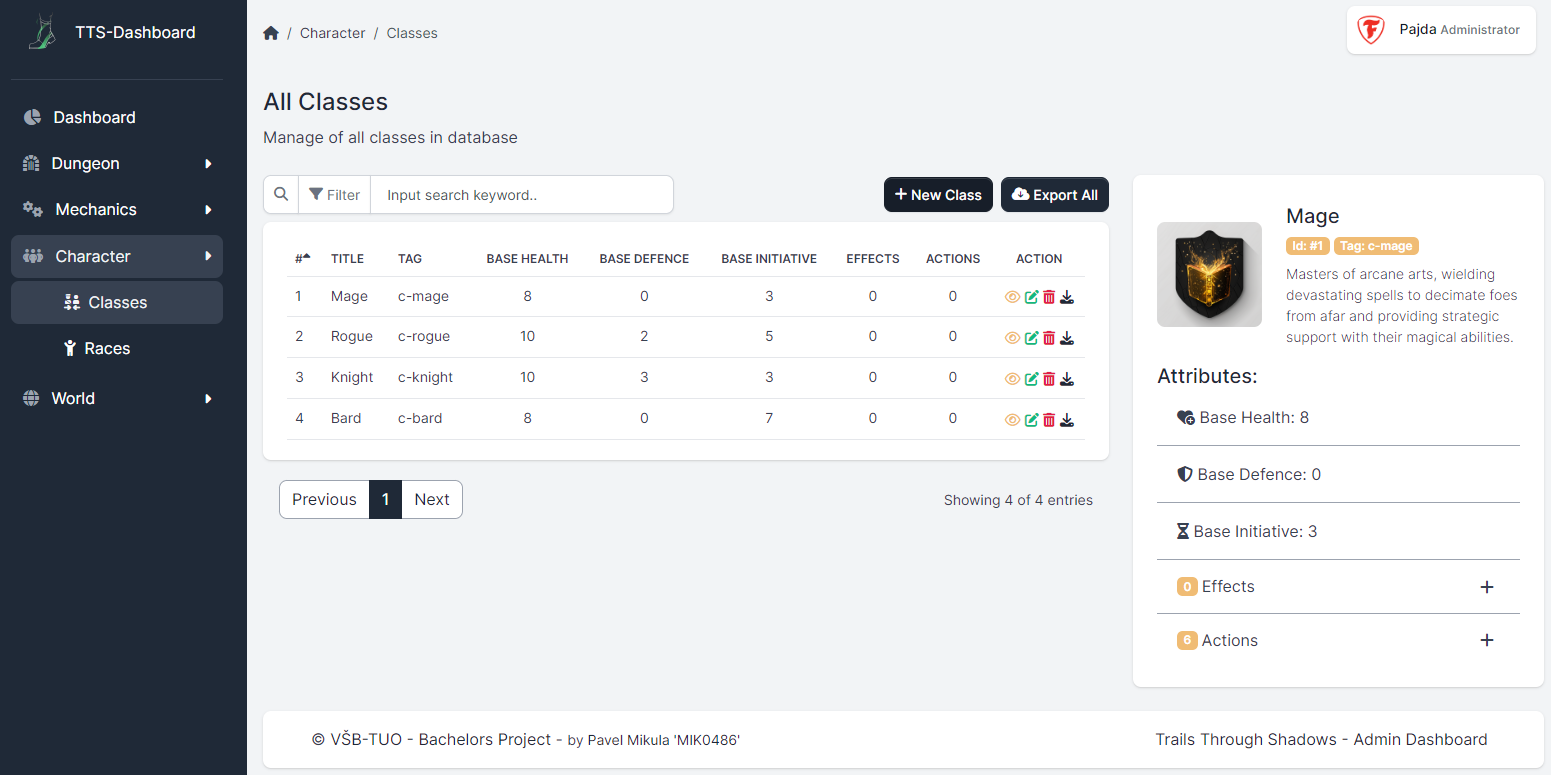
\includegraphics[width=1.0\textwidth]{figures/dashboardTable}
    \caption{Ukázka výslédného rozhraní při hledání.}
    \label{fig:interfaceScreenshotsTable}
\end{sidewaysfigure}


\begin{sidewaysfigure}[ht]
    \centering
    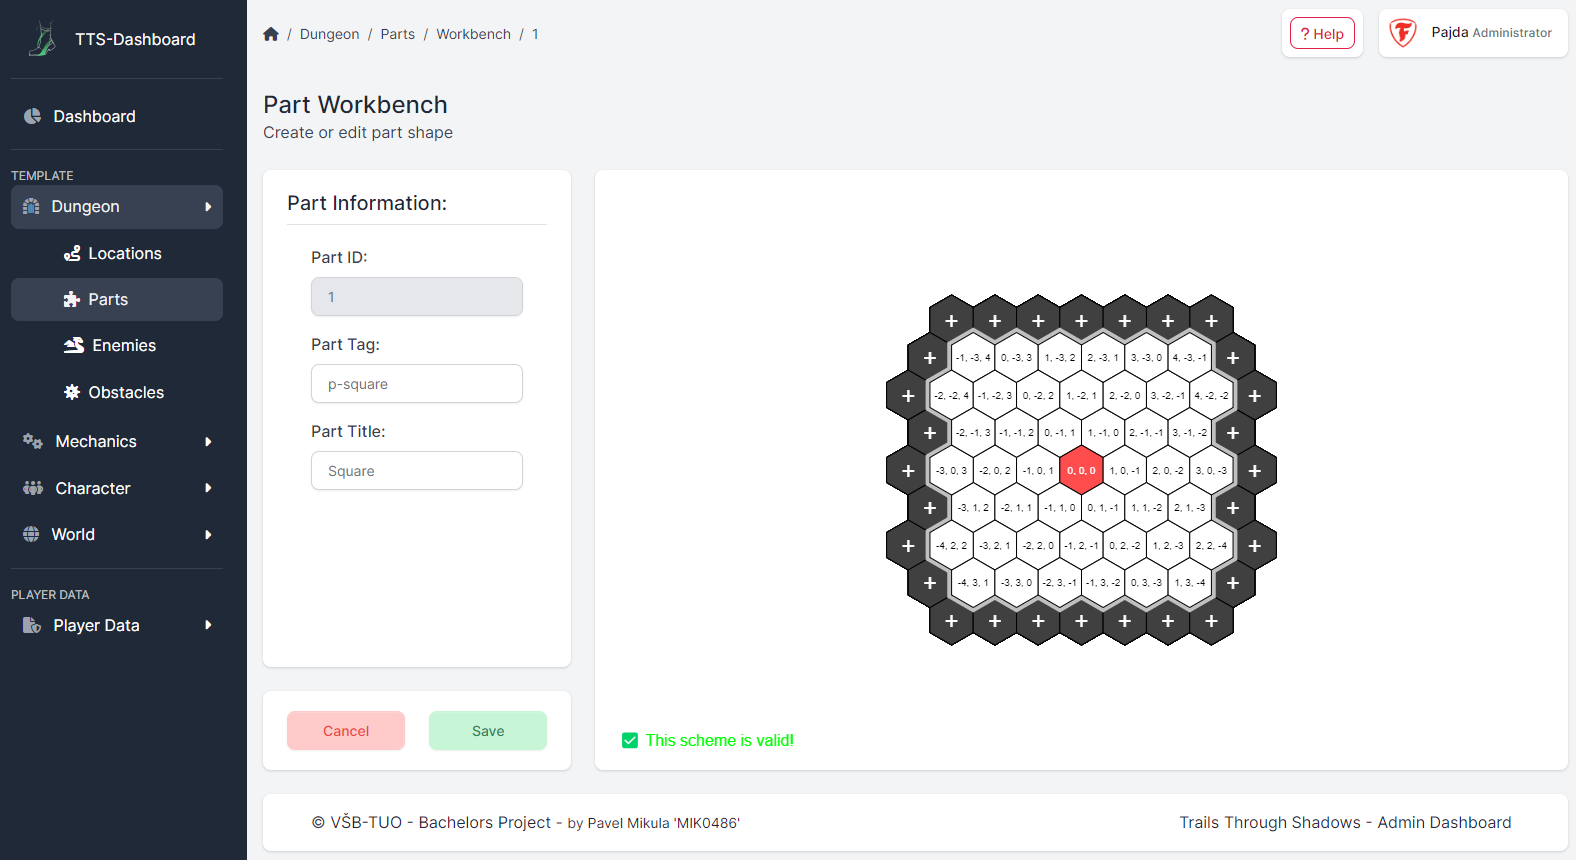
\includegraphics[width=1.0\textwidth]{figures/dashboardWorkbenchPart}
    \caption{Ukázka výslédného rozhraní při editaci partu.}
    \label{fig:interfaceScreenshotsWorkbench}
\end{sidewaysfigure}

\begin{sidewaysfigure}[ht]
    \centering
    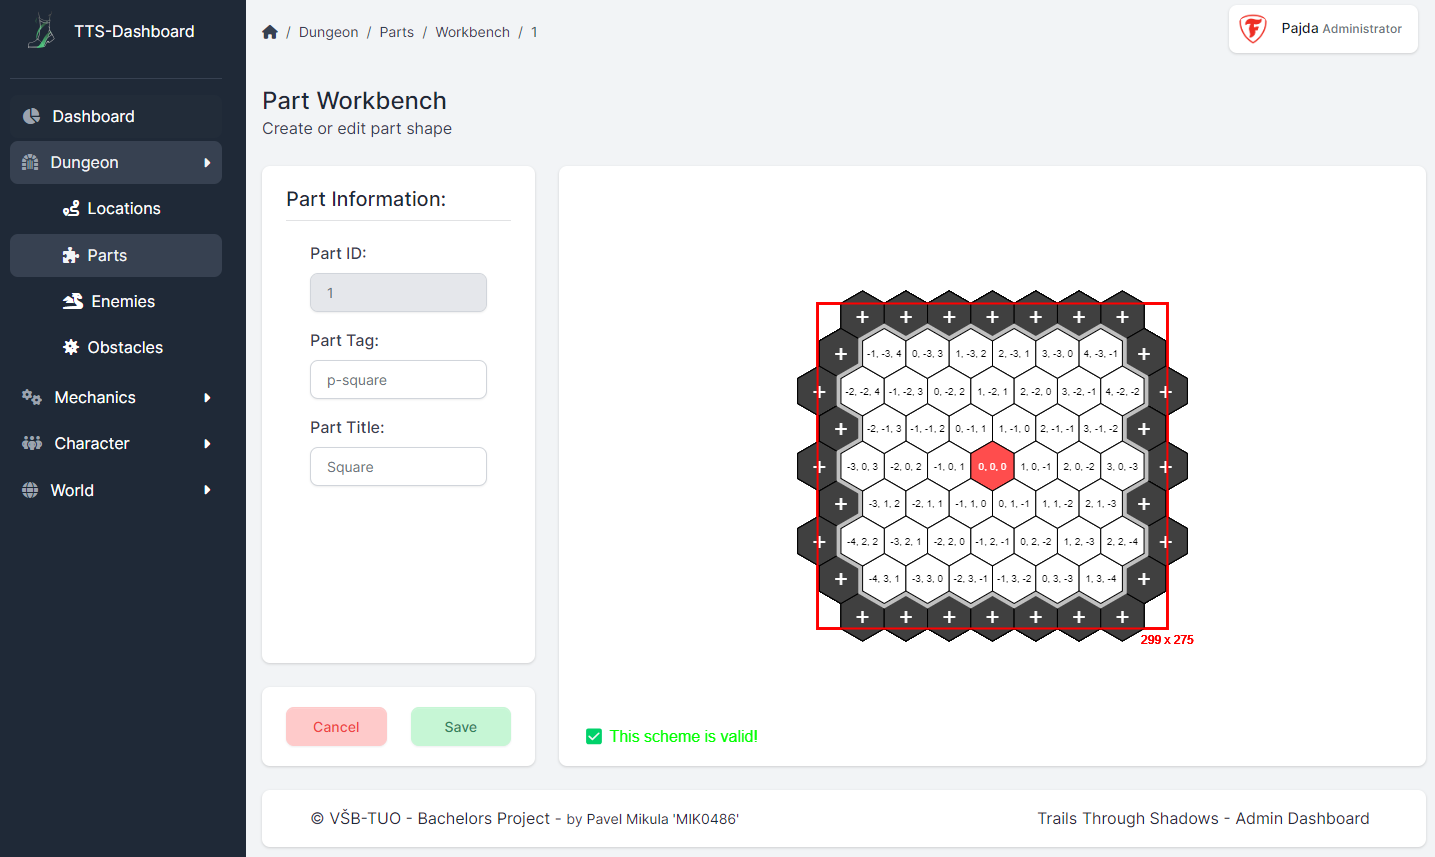
\includegraphics[width=1.0\textwidth]{figures/dashboardWorkbenchEnemy}
    \caption{Ukázka výslédného rozhraní při editaci nepřátel.}
    \label{fig:interfaceScreenshotsWorkbench2}
\end{sidewaysfigure}

\endinput